% To je predloga za poročila o domačih nalogah pri predmetih, katerih
% nosilec je Blaž Zupan. Seveda lahko tudi dodaš kakšen nov, zanimiv
% in uporaben element, ki ga v tej predlogi (še) ni. Več o LaTeX-u izveš na
% spletu, na primer na http://tobi.oetiker.ch/lshort/lshort.pdf.
%
% To predlogo lahko spremeniš v PDF dokument s pomočjo programa
% pdflatex, ki je del standardne instalacije LaTeX programov.

\documentclass[a4paper,11pt]{article}
\usepackage{a4wide}
\usepackage{fullpage}
\usepackage[utf8x]{inputenc}
\usepackage[slovene]{babel}
\selectlanguage{slovene}
\usepackage[toc,page]{appendix}
\usepackage[pdftex]{graphicx} % za slike
\usepackage{setspace}
\usepackage{color}
\definecolor{light-gray}{gray}{0.95}
\usepackage{listings} % za vključevanje kode
\usepackage{hyperref}
\usepackage{titlesec}

\renewcommand{\baselinestretch}{1.2} % za boljšo berljivost večji razmak
\renewcommand{\appendixpagename}{\normalfont\Large\bfseries{Priloge}}


\titleformat{name=\section}[runin]
  {\normalfont\bfseries}{}{0em}{}
\titleformat{name=\subsection}[runin]
  {\normalfont\bfseries}{}{0em}{}


% header
\makeatletter
\def\@maketitle{%
  \noindent
  \begin{minipage}{2in}
  \@author
  \end{minipage}
  \hfill
  \begin{minipage}{1.2in}
  \textbf{\@title}
  \end{minipage}
  \hfill
  \begin{minipage}{1.2in}
  \@date
  \end{minipage}
  \par
  \vskip 1.5em}
\makeatother


\lstset{ % nastavitve za izpis kode, sem lahko tudi kaj dodaš/spremeniš
language=Python,
basicstyle=\footnotesize,
basicstyle=\ttfamily\footnotesize\setstretch{1},
backgroundcolor=\color{light-gray},
}


% Naloga
\title{Naloga 1}
% Ime Priimek (vpisna)
\author{Andrej Hafner (63160122)}
\date{\today}

\begin{document}

\maketitle

\subsection{Podatki.}
Podatki so podani v obliki tabele, ki je vsebovala države, njihove pesmi in glasovanja na finalnem delu Evrovizije v razponu 11 let. Tabela je vsebovala nekaj atributov, ki niso relevantni in so bili zato odstranjeni (ime pesmi, izvajalec in drugo). Uporabljene so bile ocene ostalih držav za določeno pesem druge države. Število držav, torej atributov, je 47, število primerov pa je 291. Zaloga vrednosti glasov je med 0 in 12, povprečno število glasov pa je 2,5. Vsako leto se niso vse države uvrstile v finalni del, zato manjka 34\% podatkov. Za posamezno državo dobimo profil glasovanja kar kot posamezen atribut države. Ta vsebuje vse primere kako je država glasovala za ostale. Če izračunamo razdaljo med temi profili, dobimo blizu skupaj države, ki so podobno glasovale.

\section{Računanje razdalj.}
Razdalje med profili so bile izračunane z Evklidsko razdaljo, ki računa razlike med glasovanji na podlagi posameznih primerov znotraj dveh profilov. Na podlagi teh razdalj je bila ustvarjena prva gruča. Za računanje razdale med njimi je bila uporabljena povprečna Evklidska razdalja med gručami. Torej se je izračunala razdalja med vsemi elementi obeh gruč in se nato delila s številom povezav. 

V tabeli je primanjkovalo kar 34\% podatkov. Če ne bi bili umetno dodani, bi izgubili velik del podatkov. Zato je bilo za manjkajoče primere uporabljeno povprečje glasovanj iz ostalih let. Torej če v določenem letu neka država ni glasovala za drugo državo, se je ta glas nadomestil s povprečjem iz glasovanj ostalih let za par država glasovalka - glasovana država.

\section{Dendogram}
Prikazan je na sliki ~\ref{slika1}, v prilogi ~\ref{app-dendo} pa je za boljo preglednost podana še tekstovna datoteka dendograma.

\begin{figure}[htbp]
\begin{center}
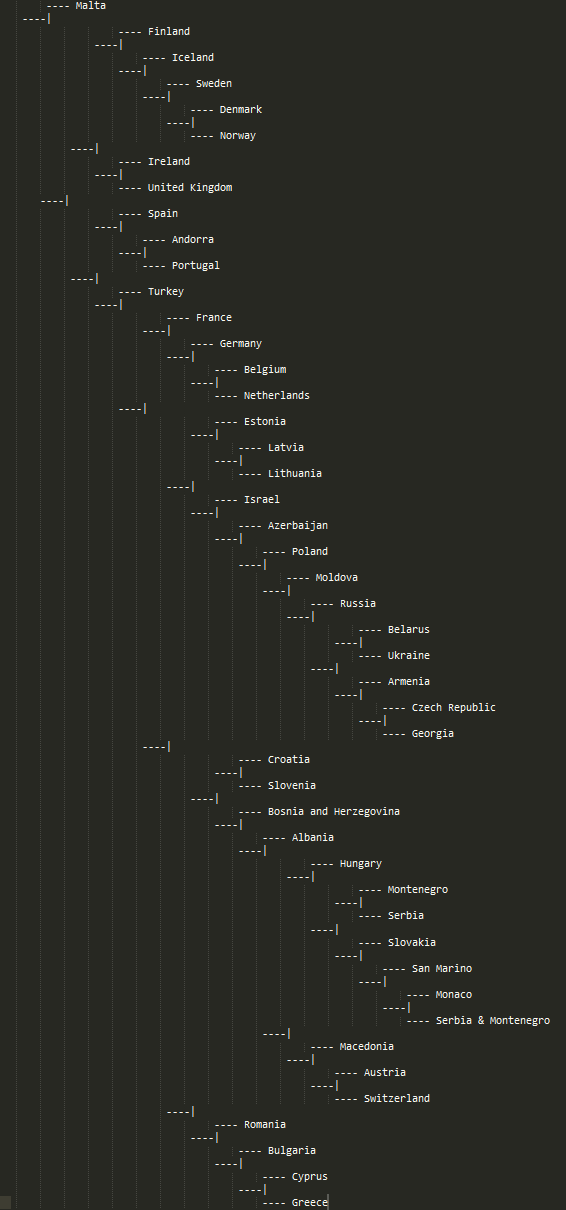
\includegraphics[scale=0.7]{dendogram-slika.png}
\caption{Tekstovni dendogram podobnosti profilov glasovanja držav.}
\label{slika1}
\end{center}
\end{figure}

\pagebreak
\section{Skupine in njihove preferenčne izbire.}
Skupine so bile oblikovane vizualno glede na vertikalni presek dendograma (razen Malte in Turčije, ki sta izstopali in sta bili dodani v zadnjo skupino). Preferiti so bili izbrani tako, da je bila vzeta država, ki je od ostalih držav dobila maksimalno število glasov.

\begin{table}[htbp]
\caption{Glasovalne skupine in njihovi preferiti .}
\label{tab1}
\begin{center}
\begin{tabular}{llp{3cm}}
\hline
skupina & države & preferiti \\
\hline
1 & Finland, Iceland, Sweden, Denmark, Norway & Sweden \\
2 & Ireland, United Kingdom & United Kingdom \\
3 & Spain, Andorra, Portugal & Spain\\
4 & France, Germany, Belgium, Netherlands & Germany\\
5 & Estonia, Latvia, Lithuania & Lithuania\\
6 & Russia, Belarus, Ukraine, Armenia,  & Russia\\
  & Czech Republic, Moldova, Georgia, Poland &  Poland\\
7 & Azerbaijan, Israel & Azerbaijan\\
8 & Romania, Bulgaria, Cyprus, Greece & Greece\\
9 & Croatia, Slovenia, Bosnia and Herzegovina & Croatia\\
10 & Albania, Hungary, Montenegro, Serbia, Slovakia & Serbia\\
  & San Marino, Monaco, Serbia \& Montenegro & \\
11 & Macedonia, Austria, Switzerland & Switzerland\\
12 & Malta, Turkey & \\
\hline
\end{tabular}
\end{center}
\end{table}


\section{Izjava o izdelavi domače naloge.}
Domačo nalogo in pripadajoče programe sem izdelal sam.

\appendix
\appendixpage
\section{\label{app-code}Programska koda.}

Priložena je programska koda v datoteki \textbf{naloga1.py} . Slednja vsebuje kodo za preprocesiranje podatkov in implementacijo hierahičnega razvrščanja.

\section{\label{app-dendo}Tekstovna datoteka dendograma.}
Za boljšo preglednost.


\end{document}
